\subsection{Base de donnée}
Nous allons créer une base de donnée en utilisant l'exemple de posts sur un blog.


\subsubsection[PHPMyAdmin][]{\phpmyadmin{}}
\phpmyadmin{} est un site/logiciel permettant à des ignares comme nou\ldots comme vous* de manipuler des bases de données facilement sans connaissances en \mysql. Pour l'instant, nous allons configurer le \verb|.env| de notre site pour acceuillir une base de donnée et ensuite créer celle-ci grâce à \phpmyadmin{} (normalement ca ca sera fait ds le tuto d'installation en fait\ldots).

\subsubsection[Models][laravel.com/docs/10.x/eloquent\#generating-model-classes]{Models}
Comme dit dans la \texttt{Section~\ref{sec:fonctionnement&philosophie}}, le \model{} est l'objet qui nous permettra d'intéragir avec les \textit{posts} stockés dans notre base de donnée\footnote{pour chaque nouvel objet, on aura un \model{} correspondant}. Pour le créer, tapez \verb|php artisan make:model Post -m|, et observez la création d'un fichier \verb|Post.php| dans \verb|app/Models/|. Pour le moment, la class (au sens \php{} du terme) est vide, mais on peut ajouter des methods spécifique à ce \model{}, ce qui, nous le verrons (WIP), est très pratique.

\subsubsection[Migrations: théorie][laravel.com/docs/10.x/migrations\#introduction]{Migrations: comme les oiseaux?}

Une \migration{} est un fichier qui permet de définir les \tables{} de notre base de donnée. Une \table{} est grosso modo un type de donnée que la \db{} va stocker. Par exemple, la liste de tous les utilisateurs est une \table{}, tout comme les \textit{posts} que nous allons créer. Chaque \table{} contient un certain nombre de \columns{} qui elles sont les données stockées en temps que telles. En l'occurence, notre \table{} de \textit{posts} doit contenir une \column{} pour le titre d'un \textit{post} et une pour son contenu en lui même\footnote{Tous ces termes sont compliqués à décrire avec des mots, mais sont en réalité très intuitifs quand on imagine les données affichées dans un grand tableau à double entrée.}.

Pour créer notre migration, tapez \verb|rien du tout| car en fait, la \migration{} a été créée en même temps que notre \model{}! Elle se trouve dans \\\verb|database/migration/xxxx_xx_xx_xxxxxx_create_posts_table.php|. \\Ensuite, remplissez là comme à la \texttt{Figure~\ref{fig:basic_migration}}\footnote{lignes 16 et 17, de rien}:

Analysons tout a:
\begin{itemize}
    \item \verb|function up()| et \verb|function down()|: La première est exécutée quand on souhaite créer les \tables{} à l'intérieur tandis que la deuxième est exécutée lorsqu'on souhaite supprimer les \tables{} de la \db{}. Pour l'utilisation simple que nous faisont des \migrations{}, pensez à \verb|down| tout ce que vous \verb|up|-per.
    \item \verb|Schema::create('posts',...| en gros, c'est la fonction utilisée pour créer la table \verb|'posts'|, et les \verb|$table->| qui suivent permettent de définir chaque \column{} de la table créée.
    \item \verb|id()|: l'id est ce qu'on appelle la \texttt{Primary Key}. Unique pour chaque \row{}\footnote{une \row{} est un élément de donnée dans une \table{}}, il permet d'identifier chaque élément de donnée. Il se trouve par défaut sur chaque \table{} nouvellement créée.
    \item \verb|string()| permet de créer une \column{} de type string, de taille 255. La taille est modifiable en ajoutant un nombre <255 en second argument.
    \item \verb|mediumtext()| permet de créer une \column{} de $16.777.215$ charactères (oula).
    \item \verb|timestamps()| ajoute une date de création et de modification à la \table{}. Ces deux \columns{} sont également ajoutées par défaut.
\end{itemize}

\begin{wrapfigure}[20]{r}{0.5\textwidth}
    \vspace{-0.5cm}
    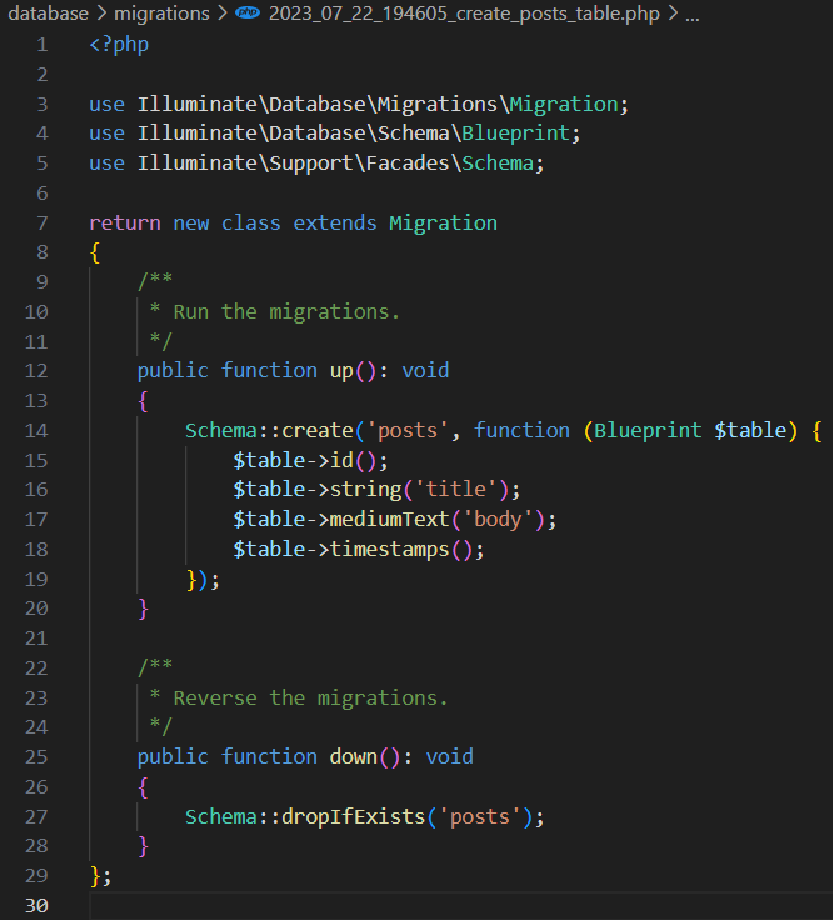
\includegraphics[width=0.5\textwidth]{figures-C1/post_migration.pdf}
    \caption{Exemple très simple de \migration{}\label{fig:basic_migration}}
\end{wrapfigure}
Quelques remarques supplémentaires:

\begin{enumerate}
    \item Par défaut, les \columns{} doivent obligatoirement posséder une valeur.
    \item On peut ajouter de nombreux paramètres aux \columns{} pour modifier leur comportements (exemple: \verb|->nullable()| pour leur permettre d'être vide).
    \item Les types des \column{} correspondent chacune à un type de valeur de \mysql{}, le ``vrai'' langage pour communiquer avec les \db{} duquel \laravel{} nous protège grâce aux \models{}, \migrations{}, \tables{} que nous venons de voir.
\end{enumerate}

Encore une fois, parcourir la doc officielle de \laravel{} permet d'en apprendre beaucoup plus que ce que tutoriel ne pourra jamais vous apprendre!

\subsubsection[Migrations: exécution]{Migrations: exécution}

Bon, après tant de blabla, passons à l'action. Mais avant cela, \laravel{} nous embête (pour une fois). Afin de n'avoir aucune erreur en exécutant la migration, il va falloir ajouter ces lignes dans \verb|app/Providers/AppServiceProvider.php|:

\begin{figure}[!h]
    \centering
    \begin{minipage}{0.49\textwidth}
         \centering
         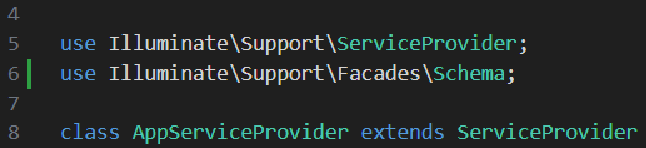
\includegraphics[width=\textwidth]{figures-C1/appservice_2.pdf}
    \end{minipage}
    \begin{minipage}{0.49\textwidth}
         \centering
         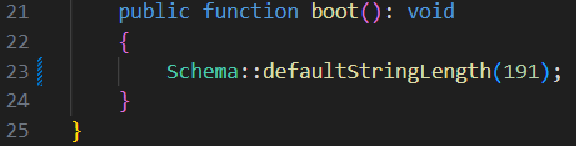
\includegraphics[width=0.95\textwidth]{figures-C1/appservice_1.pdf}
    \end{minipage}
\end{figure}

Voilà! maintenant tapez \verb|php artisan migrate:fresh --seed| (où \verb|fresh| signifie que tout ce qui existait avant est supprimé et \verb|--seed| permet d'exécuter les \texttt{seeders} vus dans la \texttt{Section~} (WIP)) et, si tout va bien, vous verrez maintenant cela en allant dans \phpmyadmin{}:

\begin{figure}[!h]
    \centering
    \begin{minipage}{0.49\textwidth}
         \centering
         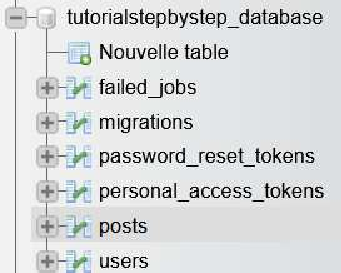
\includegraphics[width=0.6\textwidth]{figures-C1/db_posts_1.pdf}
    \end{minipage}
    \begin{minipage}{0.49\textwidth}
         \centering
         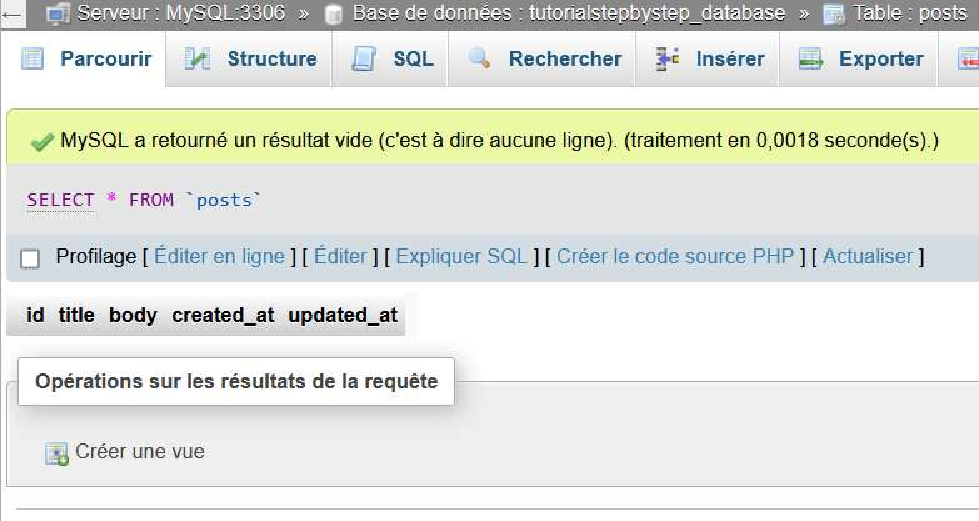
\includegraphics[width=0.9\textwidth]{figures-C1/db_posts_2.pdf}
    \end{minipage}
\end{figure}

\subsubsection[PostsController][laravel.com/docs/10.x/controllers\#resource-controllers]{PostsController}

Pour gérer ces posts, nous allons bien entendu avoir besoin d'un \controller{}. Comme ce genre de donnée va avoir des manipulations basiques très communes (création, liste, affichage, modification, suppression,\ldots), il existe un certain type de controller permettant de nous faire gagner du temps: le \texttt{resource} \controller{}. Tapez donc \\
\verb|php artisan make:controller PostsController --resource| pour en créer un.

Ensuite, il faut évidement définir des nouvelles routes. Une seule ligne toute simple nous permet de générer en réaliter 7 \routes{} différentes que nous verrons petit à petit. Ajoutez donc ces 2 lignes dans \verb|routes/web.php|:

\begin{figure}[!h]
    \centering
    \begin{minipage}{0.6\textwidth}
        \centering
        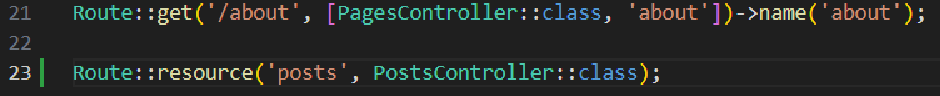
\includegraphics[width=\textwidth]{figures-C1/res_route_1.pdf}
        \caption{\label{fig:post_route}}
    \end{minipage}
    \begin{minipage}{0.38\textwidth}
        \centering
        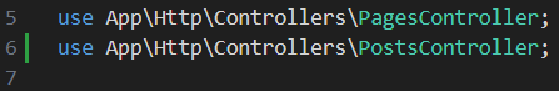
\includegraphics[width=\textwidth]{figures-C1/res_route_2.pdf}
        \caption{}
    \end{minipage}
\end{figure}
\vspace{-0.5cm}
Notez que en donnant \textit{'posts'} en argument à \verb|resource()|, celui-ci fait automatiquement lien avec le \model{} \verb|Post|\footnote{Pour comprendre comment \laravel{} fait pour être si intelligent, jetez un oeil à \href{https://laravel.com/docs/10.x/eloquent#table-names}{ceci}.}.

Petite parenthèse avant de continuer: un exemple de route générée par la commande de la \texttt{Figure~\ref{fig:post_route}} est: \\
\verb|Route::get('/posts/{post}', [PostsController::class, show])->name('posts.show')|
le \verb|{...}| dans l'URL est une sorte de paramètre dans l'URL, qui permet de passer des informations au controller. En effet, chaque paramètre dans l'URL sera passé (si on le souhaite) en argument aux fonctions du controller, dans le même ordre d'apparition que dans l'URL. Ce paramètre est extrêmement utile comme nous le verrons à la \texttt{Section~\ref{sec:post_show}}. Fin de la parenthèse.

Bon, maintenant, il faut remplir ce \controller{} et créer les \views{} qui vont avec. Commençons par les plus simples, \verb|index()| et \verb|show()|.

\subsubsubsection{index}
Cette method est utilisée pour afficher la liste de tous les Posts créés. 

\begin{wrapfigure}[5]{r}{0.4\textwidth}
    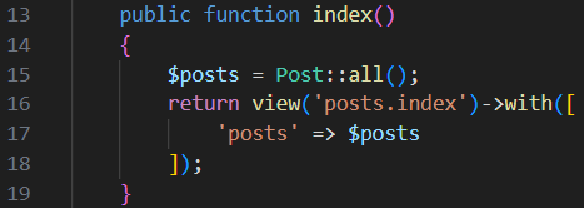
\includegraphics[width=0.4\textwidth]{figures-C1/post_index_controller.pdf}
\end{wrapfigure}
Avec cet exemple simple, on comprend vite à quel point il est simple d'intéragir avec la \db{} par l'intermédiaire des \models{}. Nos posts sont stockés sous forme d'une array d'objets \php{}, contenant les champs que nous avons spécifés dans la \migration{}. 

\SaveVerb{post_index}|index.blade.php|
\begin{wrapfigure}[11]{r}{0.581\textwidth}
    \vspace{-0.5cm}
    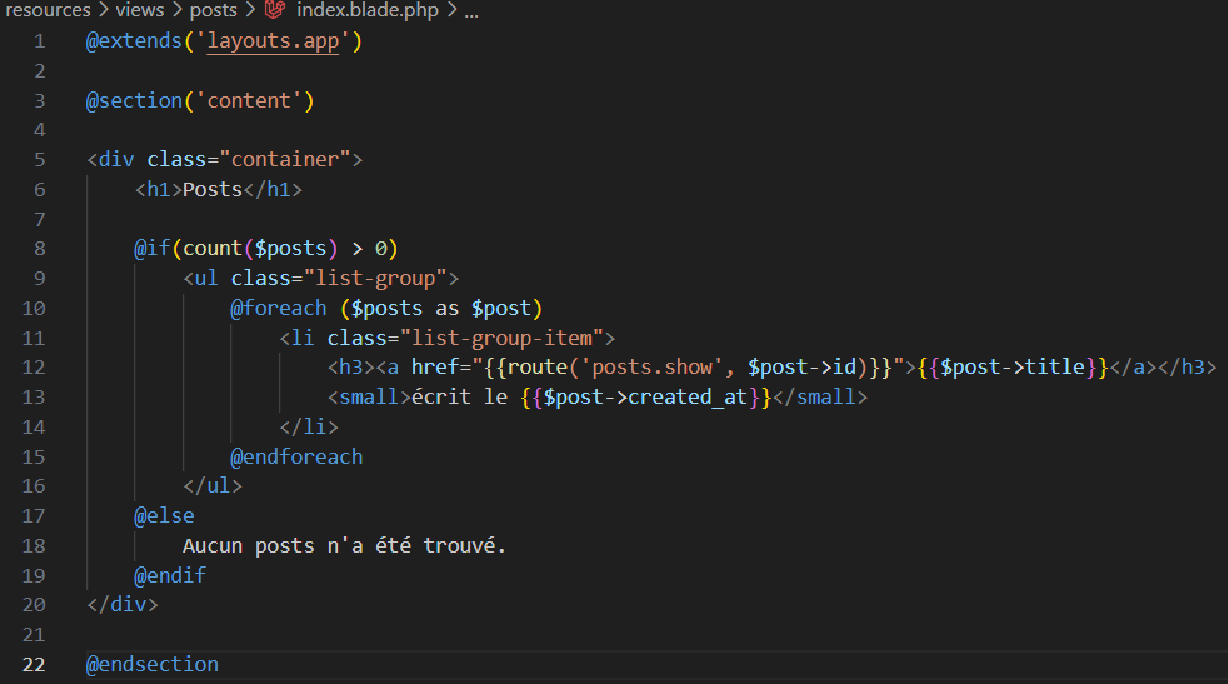
\includegraphics[width=0.581\textwidth]{figures-C1/post_index_blade.pdf}
    \caption{\protect\UseVerb{post_index}\label{fig:post_index}}
\end{wrapfigure}
Ensuite, nous allons créer un nouveau dossier \verb|posts| dans  \\ \verb|resources/views| et ajouter un fichier dedans appelé \\ \verb|index.blade.php|. Il ne reste ``plus qu'à'' le remplir avec le contenu de la \texttt{Figure~\ref{fig:post_index}}.

Ici, tout est déjà connu mis à part le \verb|@if|, mais c'est plutôt intuitif au vu de ce que je vous ai déjà appris. Ensuite, il y a le \verb|->| permettant d'accéder aux différents champs des objets que sont nos \verb|$post|.

Enfin, il ne nous reste plus qu'à ajouter un bouton à notre navbar afin d'accéder à cette page.

\begin{figure}[!h]
    \centering
    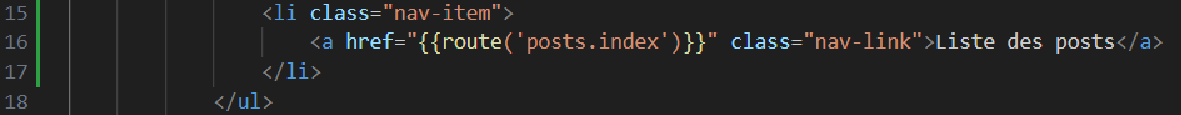
\includegraphics[width=0.75\textwidth]{figures-C1/post_index_navbar.pdf}
\end{figure}

\subsubsubsection{show}\label{sec:post_show}

Même chose que pour la page précédente, il faut remplir la fonction \verb|show()|.

\begin{wrapfigure}[5]{r}{0.4\textwidth}
    \vspace{-0.5cm}
    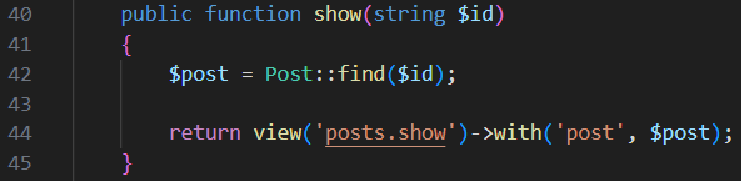
\includegraphics[width=0.4\textwidth]{figures-C1/post_show_controller.pdf}
\end{wrapfigure}
Ici, nous utilisons ce que j'ai expliqué en dessous de la \texttt{Figure~\ref{fig:post_route}}. La fonction \verb|show()| prend un argument, appelé \verb|$id|. Pourquoi et d'où sort-il? Son origine a été expliquée plus haut, il provient du paramètre \verb|{post}| dans l'URL correspondant à la fonction\footnote{Si on avait eu deux paramètres différents, par exemple \verb|.../{post}/{comment}|, et qu'on avait gardé \verb|show($id1)|, \verb|$id1| aurait pris la valeur de \verb|{post}|. Pour obtenir la valeur du deuxième paramètre on aurait du écrire \verb|show($id1, $id2)| (et \verb|$id2| aurait pris la valeur de \verb|{comment}|).}. 

Maintenant, pourquoi l'avoir appellé \verb|$id|? Simplement parce qu'il contient l'ID du post que nous souhaitons obtenir, puisque c'est la valeur que nous lui avons donné en écrivant \\ \verb|route(posts.show, $post->id$)| dans la \texttt{Figure~\ref{fig:post_index}}\footnote{Le nom du paramètre dans l'URL n'a donc aucun rapport avec le nom de la variable dans la fonction, si ce n'est que l'un donne sa valeur à l'autre}. 

\textit{\underline{PS:}} L'écriture un petit peu différente du \verb|->with()| permet de simplifier l'écriture que nous avons utilisée jusqu'ici lorsque qu'il n'y a qu'un seul élément à ajouter.

Enfin, la \view{} corresondante peut être créée au nom et emplacement \verb|resources/views/posts/show.blade.php|:

\begin{figure}[!h]
    \centering
    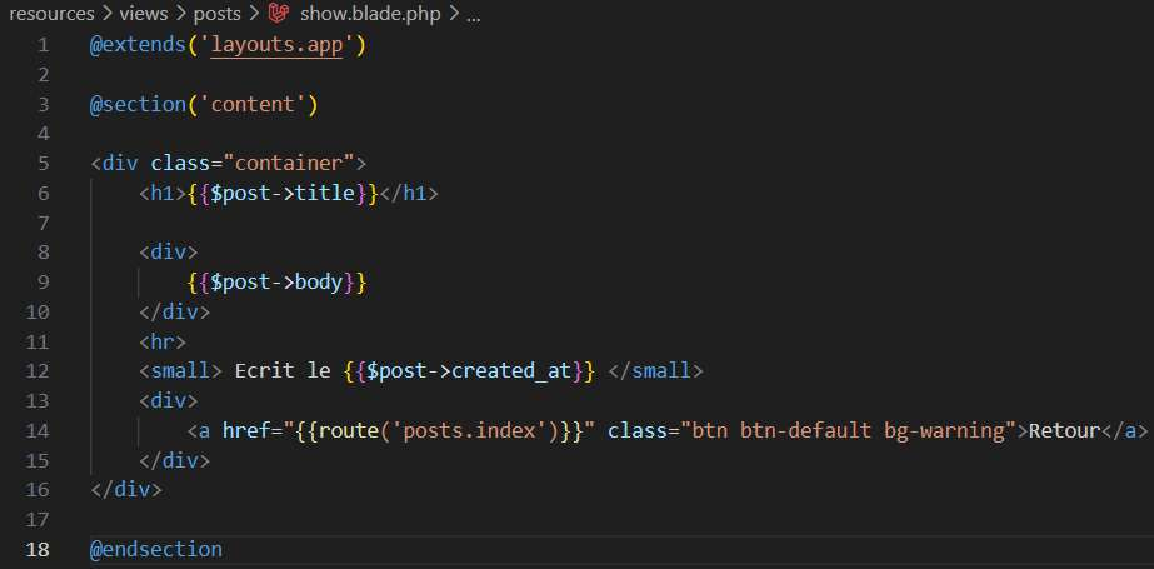
\includegraphics[width=0.75\textwidth]{figures-C1/post_show_blade.pdf}
\end{figure}

Pour le coup, R.A.S. en terme de nouveautées donc nous pouvons maintenant passer à la création de posts!

\subsubsubsection{create}

Cette partie est plus intéressante car elle va amener un nouveau concept, les \forms{}. Jusque ici, nous n'avons jamais eu à rentrer nous mêmes des données et à les envoyer à notre site pour qu'il fasse des choses avec, c'est exactement à cela que servent les \forms{}.

\begin{wrapfigure}[5]{r}{0.4\textwidth}
    \vspace{-0.5cm}
    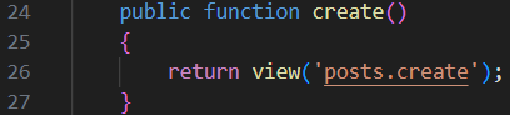
\includegraphics[width=0.4\textwidth]{figures-C1/post_create_controller.pdf}
\end{wrapfigure}
Tout d'abord, remplissons la méthode \verb|create()| du controller et créons le fichier \\ \verb|resources/posts/create.blade.php| comme nous en avons maintenant l'habitude.

Maintenant, il faut remplir la \view:

\begin{figure}[!h]
    \centering
    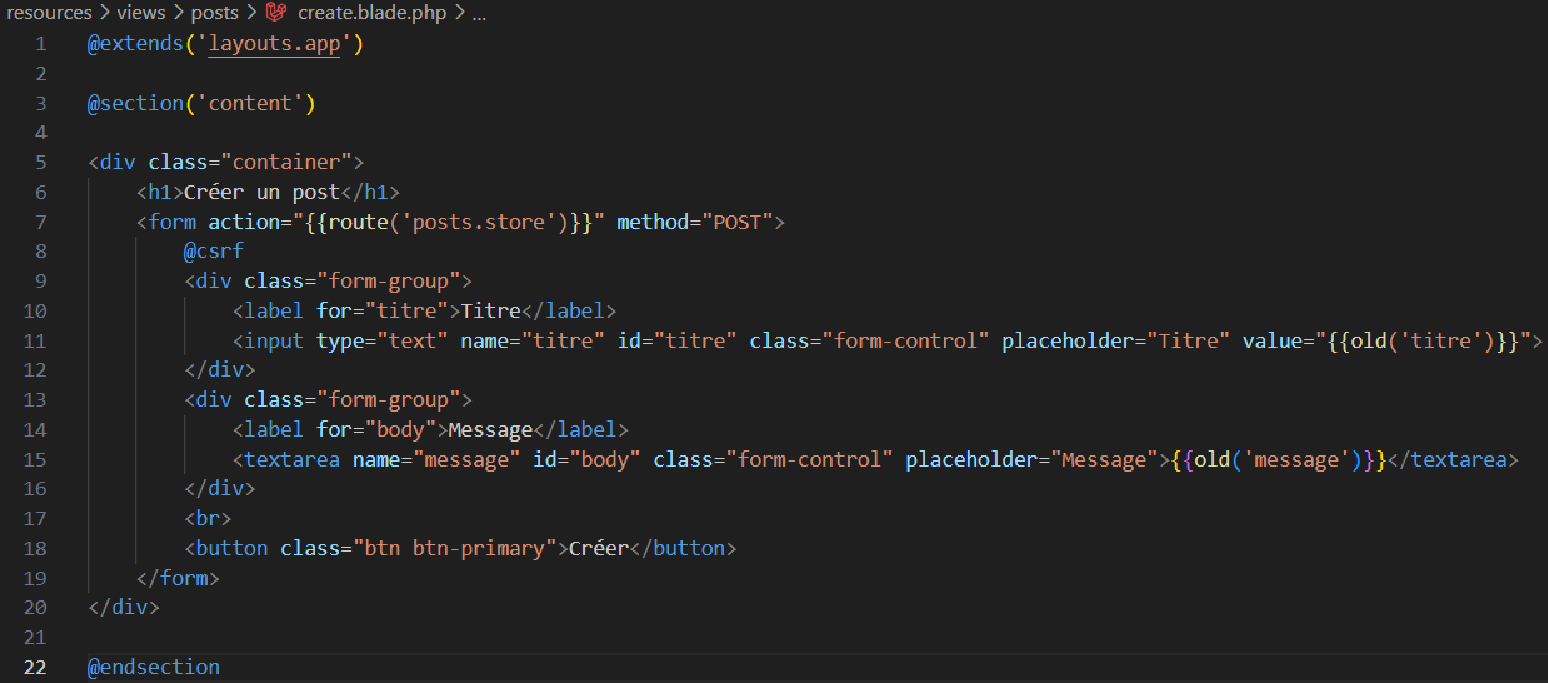
\includegraphics[width=0.8\textwidth]{figures-C1/post_create_blade.pdf}
\end{figure}
Ici il y'a pas mal de nouveautés. On voit en effet apparaitre trois nouveaux tags \html:

\begin{enumerate}
    \item \verb|<form>|: Le \form{} permet donc l'envoit d'information entrées par l'utilisateur. Pour cela, on doit lui fournir l'URL vers laquelle aller lorsque le \form{} est envoyé, c'est ce que l'on met dans \verb|action|. En l'occurence, le \texttt{resource controller} nous a créé une \route{} pour cela, appelée \verb|'posts.store'| et qui permettra de stocker les informations du \form{}. Nous verrons cela en détail à la prochaine section. Ensuite, il faut préciser le type de requête effectuée, et lorsque l'on stocke quelque chose, c'est une requête \verb|POST|\footnote{Pour afficher une \view, on utilisait des requêtes \verb|GET|.\ \href{https://developer.mozilla.org/fr/docs/Web/HTTP/Methods}{Pour en savoir plus}}
    \item \verb|<label>|: Celui-ci est simplement utilisé pour donner un nom\footnote{un nom visible sur la page internet.} à un champ \verb|<input>|. Il suffit de spécifier à quel champ le \verb|<label>| fait référence en mettant le \verb|id| de l'\verb|<input>| dans l'attribut \verb|for| du \verb|<label>|.
    \item \verb|<textarea>|: Il fonctionne comme un \verb|<input>| mais est spécialisé pour la gestion de paragraphes. L'attribut \verb|value| est quant à lui substitué par l'espace entre les deux marqueurs \verb|<textarea>| et \verb|</textarea>|.
    \item \verb|<input>|: Enfin, ce tag correspond à un champ à remplir. Ce champ peut prendre plusieurs formes qui s'indiquent au moyen de l'attribut \verb|type|. En l'occurence nous utilisons un champ \verb|text| pour une petite phrase/mots (ici, le titre de notre post)\footnote{Il existe de nombreux autres types pour des fichiers, dates, boites à cocher, \ldots vous les trouverez \href{https://developer.mozilla.org/en-US/docs/Web/HTML/Element/input#input_types}{ici}.}. Les \verb|<input>| peuvent posséder de \href{https://developer.mozilla.org/en-US/docs/Web/HTML/Element/input#attributes}{très nombreux attributs}, ici nous utilisons les attributs:
    \begin{itemize}
        \item \verb|name| qui donne le nom de la variable accessible dans le \controller{}, qui contiendra les données envoyées par cet \verb|<input>|.
        \item \verb|placeholder| qui permet d'afficher un petit texte en fond dans le champ (pour par exemple donner un format de réponse)
        \item \verb|value| qui permet de donner une valeur prédéfinie au champ lorsque l'on affiche la page. Ici, \verb|old()| est une fonction prenant en argument le nom d'un \verb|<input>| et qui permet d'afficher la valeur du champ (si elle existait\footnote{on peut donner en deuxième argument à la fonction un texte à afficher lorsque le champ était vide à la requête prcédente.}) lors de la requête précédente. C'est utile lorsque les données doivent être validées avant d'être stockées (ex: est-ce que tous les champ remplis?) et que l'utilisateur est renvoyé vers la page de saisie du \form{} si la validation échoue.
    \end{itemize}
\end{enumerate}
La dernière commande inconnue est le \verb|@csrf|. C'est une mesure de sécurité contre un certain type d'attaque. Plus d'information \href{https://laravel.com/docs/10.x/csrf}{ici}.

Bon, ce fût beaucoup (trop) de bla-bla, mais on va (enfin) pouvoir passer à la suite! Promis, les trois dernières méthodes seront bien plus simples. Mais avant cela, ne pas oublier d'ajouter un bouton sur notre navbar pour accéder à cette page:

\begin{figure}[!h]
    \centering
    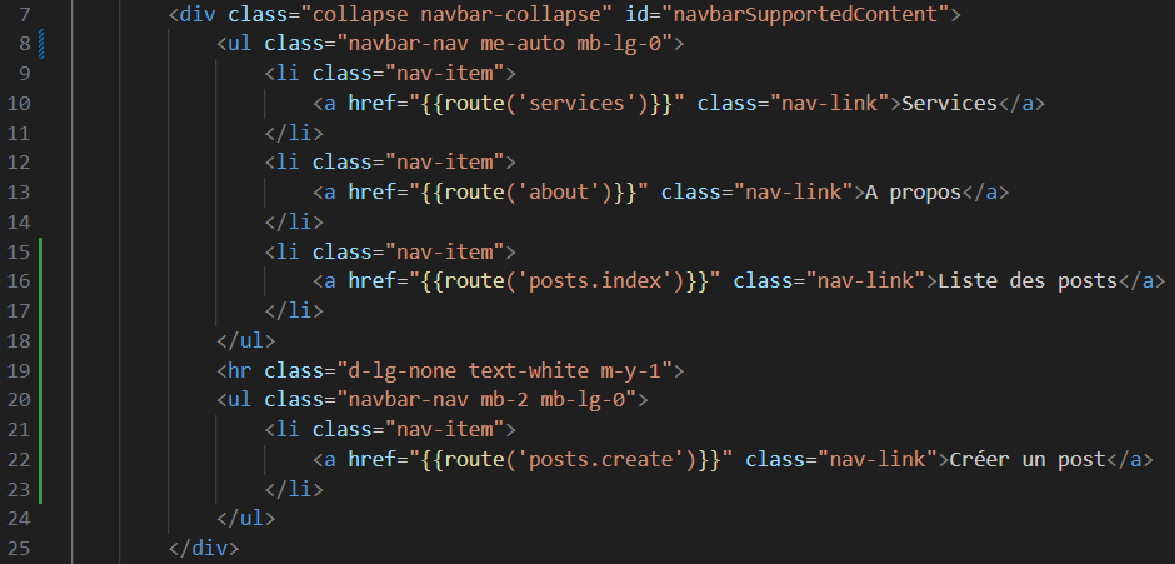
\includegraphics[width=0.75\textwidth]{figures-C1/post_create_navbar.pdf}
\end{figure}

\newpage

\subsubsubsection{store}\label{sec:posts_store}

On a vu à la section précédente que les données du \form{} étaient envoyées à la route \verb|'posts.store'|, or cette \route{} redirige vers cette fonction! C'est donc ici que nous allons stocker le post nouvellement créé.

Tout d'abord, nous allons vérifier si les 2 champs \verb|titre| et \verb|message| ont bien été remplis (s'ils doivent être remplis, ils sont requis $\Rightarrow$ \verb|required|). Pour cela, on utilise la fonction \verb|validate()| de \laravel\footnote{Plus d'informations ainsi que la liste des règles de \texttt{validation} \href{https://laravel.com/docs/10.x/validation#quick-writing-the-validation-logic}{ici}.}. Si la \texttt{validation} rate, l'utilisateur est renvoyé à la page précédente et si elle réussit, alors on continue.

\begin{wrapfigure}[9]{r}{0.7\textwidth}
    \vspace{-0.5cm}
    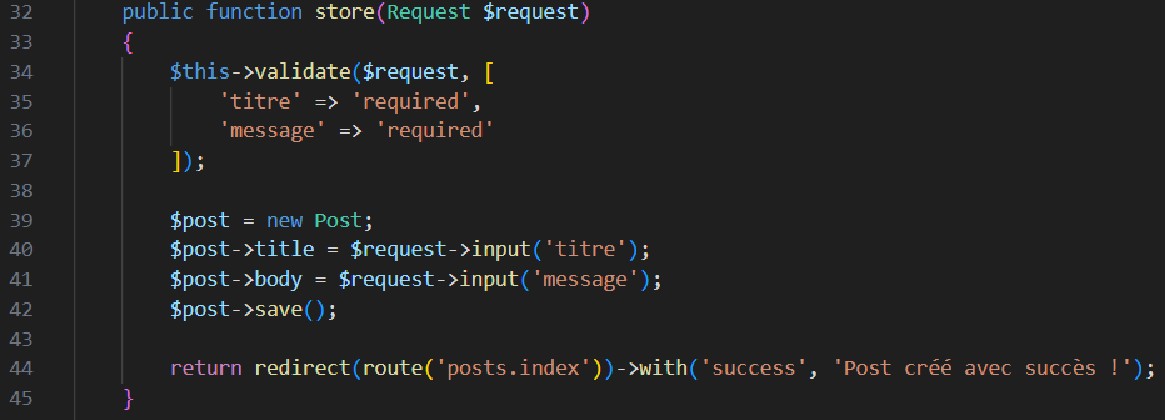
\includegraphics[width=0.7\textwidth]{figures-C1/post_store_controller.pdf}
\end{wrapfigure}
L'étape suivante est de créer un nouveau post, via son \model{}. Ensuite, on remplit ses champs avec les valeurs obtenues dans le \form{} et on le sauvegarde dans la base de donnée. Enfin, il ne reste plus qu'à envoyer l'utilisateur quelque part (la liste des posts) et le tour est joué!\footnote{La variable \verb|'success'| sera utilisée dans la \texttt{Section~\ref{sec:messages}}} Plus qu'à rajouter les fonctionnalités de modification et de suppression et puis nous en aurons terminé.

\newpage

\subsubsubsection{edit}

\begin{wrapfigure}[2]{r}{0.5\textwidth}
    \vspace{-0.5cm}
    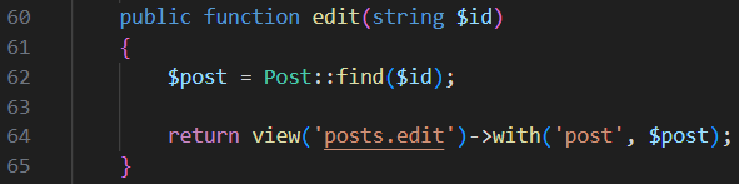
\includegraphics[width=0.5\textwidth]{figures-C1/post_edit_controller.pdf}
\end{wrapfigure}
Pour l'édition, c'est plutôt simple. Tout d'abord remplissons la méthode du \controller{}:
\vspace{1.5cm}

Ensuite, créons la \view{} dédiée:
\begin{figure}[!h]
    \centering
    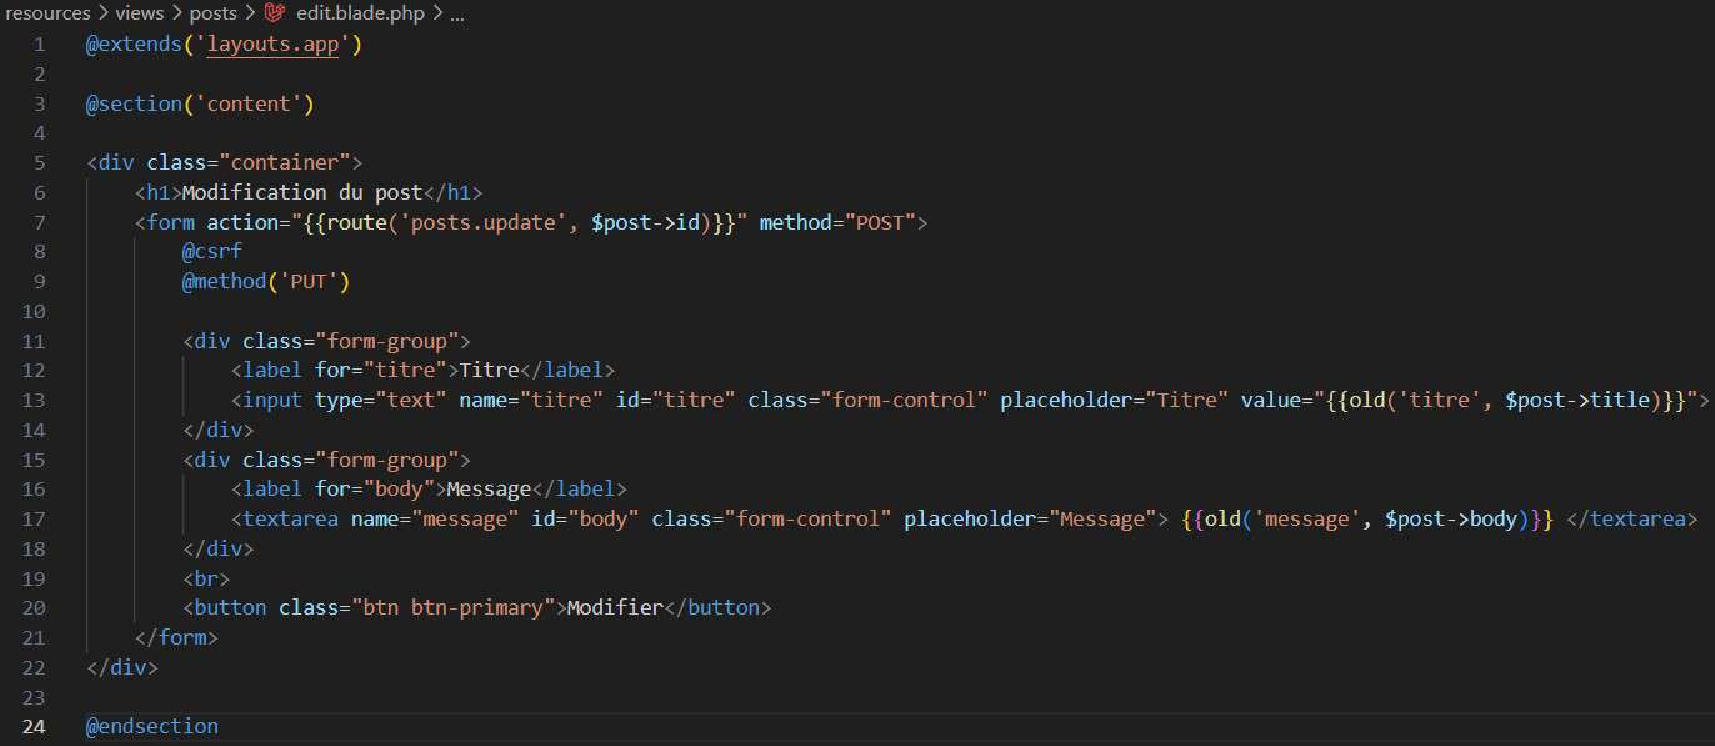
\includegraphics[width=0.75\textwidth]{figures-C1/post_edit_blade.pdf}
\end{figure}

Remarquez qu'il n'y a presque aucune différence avec la \view{} de création de post, et c'est bien normal: on peut l'utiliser quasi à l'identique à condition de mettre les valeurs du post dans les bons champs lorsque l'on accède à la page. Une différence est néanmoins à noter, la présence du \verb|@method('PUT')|. Cette méthode permet de remplacer une donnée par une autre (notre post à modifier), mais elle n'est pas disponible directement dans les \forms{}. Il faut donc effectuer une petite accrobatie pour l'utiliser.

\subsubsubsection{update}\label{sec:posts_update}

\begin{wrapfigure}[8]{r}{0.65\textwidth}
    \vspace{-0.5cm}
    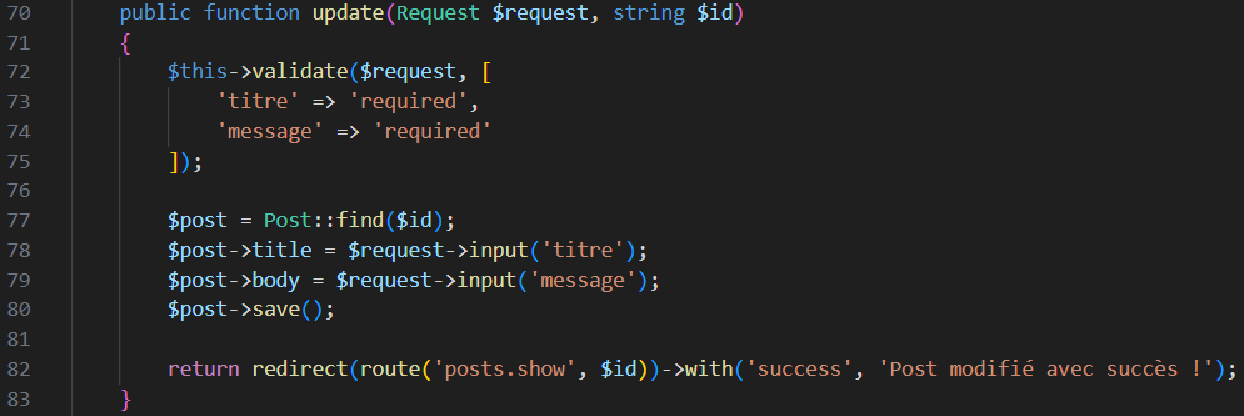
\includegraphics[width=0.65\textwidth]{figures-C1/post_update_controller.pdf}
\end{wrapfigure}
Lorsque le \form{} est envoyé, il faut bien sûr enregistrer le post dans notre \db{}. La route \verb|'posts.update'| nous envoit donc vers la méthode \verb|update()| que vous pouvez remplir comme ci-contre. Notez que ici aussi, la démarche est la même que pour la création de post (et c'est logique), mis à part qu'on cherche le post à modifier au lieu d'en créer un nouveau.

\subsubsubsection{delete}\label{sec:posts_delete}

Enfin, la suppression de post. Tout d'abord, ajoutons un bouton dans \verb|posts/show.blade.php| qui permet d'accéder à notre page de modification d'un post, un autre qui permettra de le supprimer, et stylisons un peu ces trois boutons afin qu'ils soient plaisant à voir (\texttt{Figure~\ref{fig:post_delete_blade}})

\begin{wrapfigure}[4]{r}{0.65\textwidth}
    \vspace{-0.5cm}
    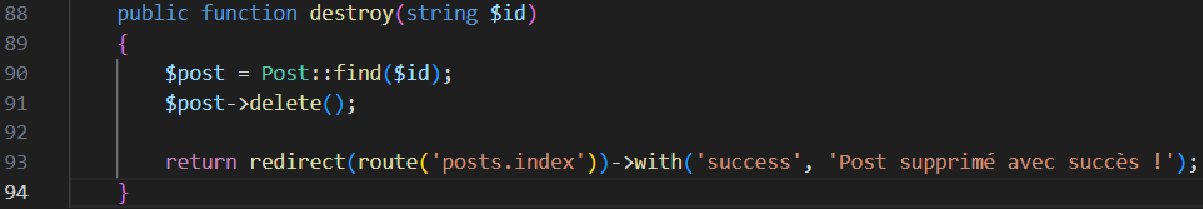
\includegraphics[width=0.65\textwidth]{figures-C1/post_delete_controller.pdf}
\end{wrapfigure}
Ensuite, remplissons la méthode du \controller{}. La mécanique est ici triviale, il suffit de sélectionner le post que l'on souhaite et ensuite de le supprimer.

\begin{figure}[!h]
    \centering
    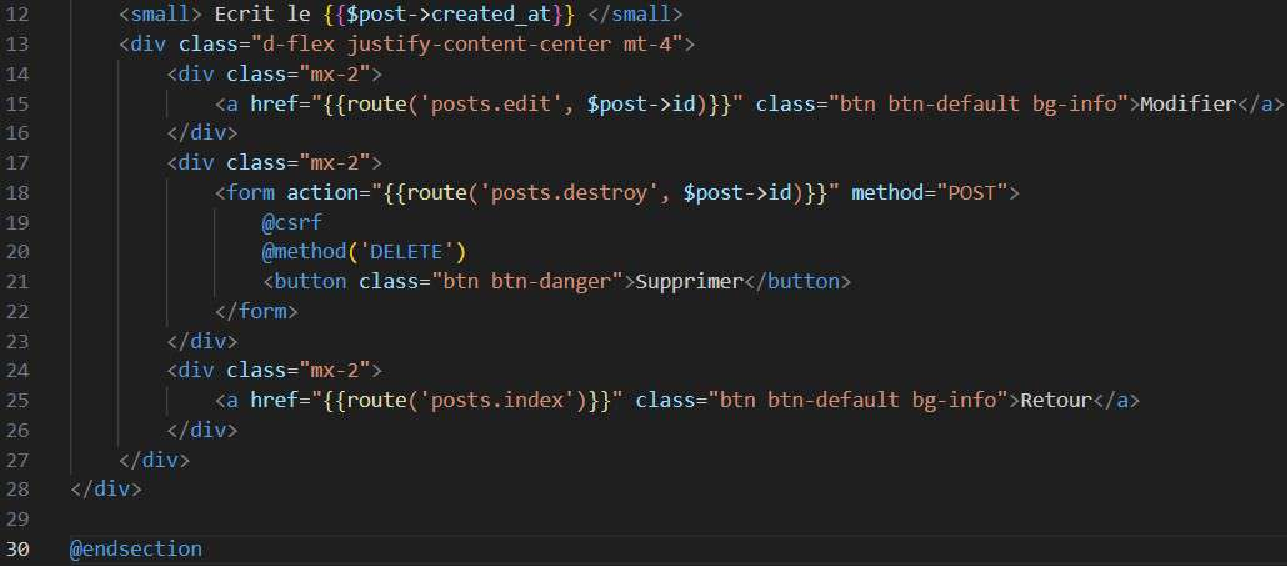
\includegraphics[width=0.75\textwidth]{figures-C1/post_delete_blade.pdf}
    \caption{\label{fig:post_delete_blade}}
\end{figure}

Et voilà! Nous avons désormais un système (simple) de création et gestion de posts! Evidément, nous pourrions rajouter énormément de fonctionnalités (commentaires, auteurs, images, \ldots). Nous explorerons certaines de ces options dans de futures sections, pour cette introduction, c'est déjà plus que suffisant.

A titre d'indication, voici le résultat auquel vous devriez arriver si tout fonctionne correctement:

\begin{figure}[!h]
    \begin{subfigure}[c]{0.73\textwidth}
        \fbox{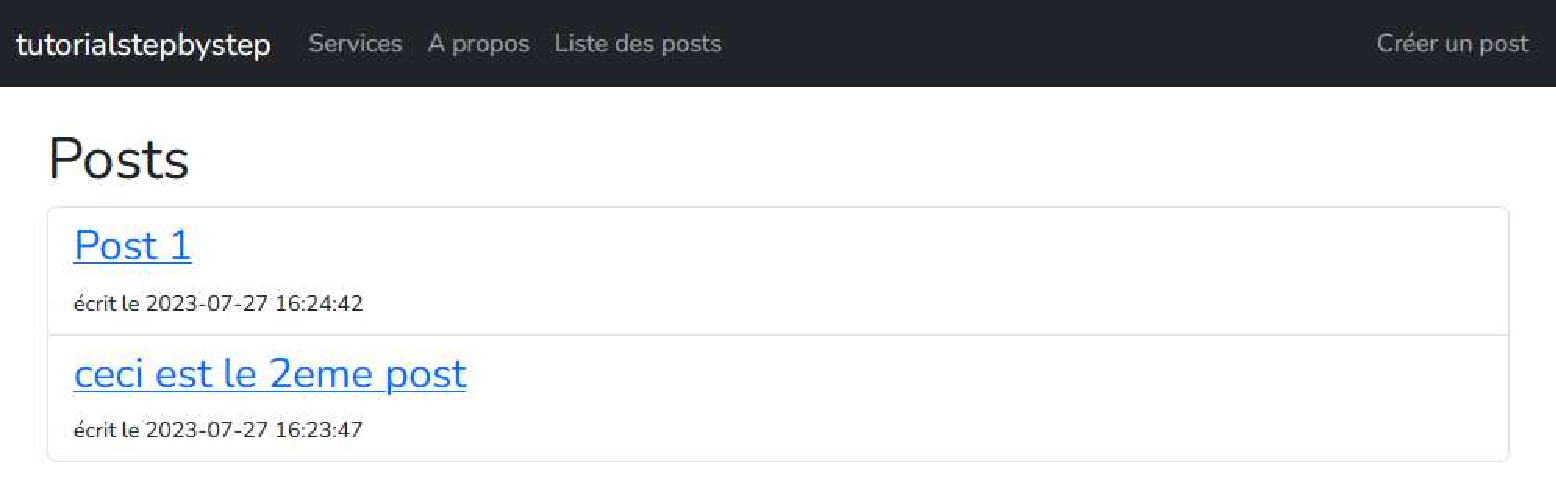
\includegraphics[width=\textwidth]{figures-C1/posts_index.pdf}}
    \end{subfigure}\hfill
    \begin{subfigure}[c]{0.24\textwidth}
        \caption{\url{http://tutorialstepbystep/posts}} 
    \end{subfigure}
    \begin{subfigure}[c]{0.73\textwidth}
        \fbox{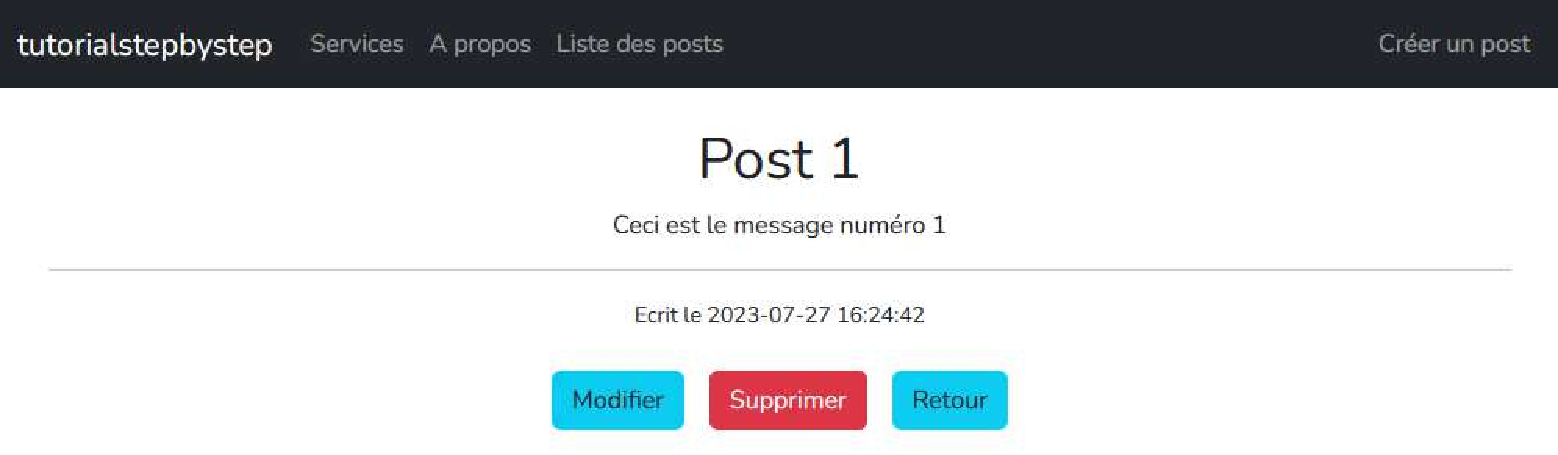
\includegraphics[width=\textwidth]{figures-C1/posts_show.pdf}}
    \end{subfigure}\hfill
    \begin{subfigure}[c]{0.24\textwidth}
        \caption{\url{http://tutorialstepbystep/posts/1}} 
    \end{subfigure}
    \begin{subfigure}[c]{0.73\textwidth}
        \fbox{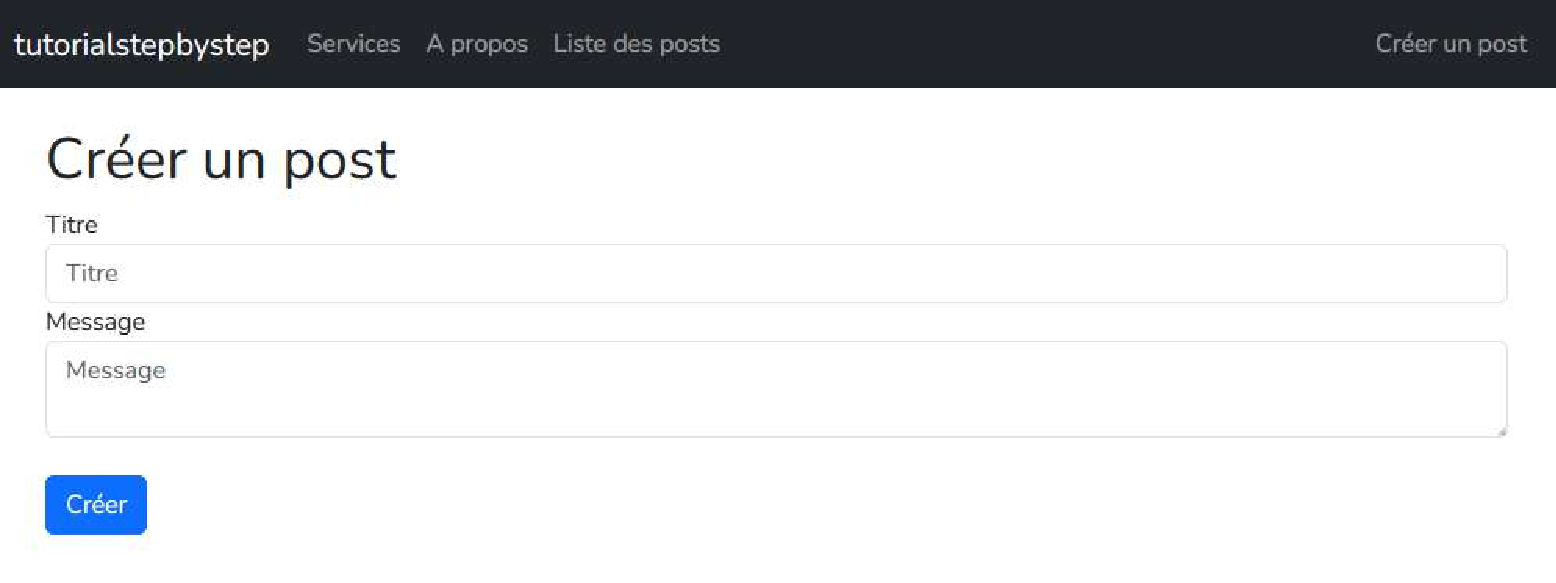
\includegraphics[width=\textwidth]{figures-C1/posts_create.pdf}}
    \end{subfigure}\hfill
    \begin{subfigure}[c]{0.24\textwidth}
        \caption{\url{http://tutorialstepbystep/posts/create}} 
    \end{subfigure}
    \begin{subfigure}[c]{0.73\textwidth}
        \fbox{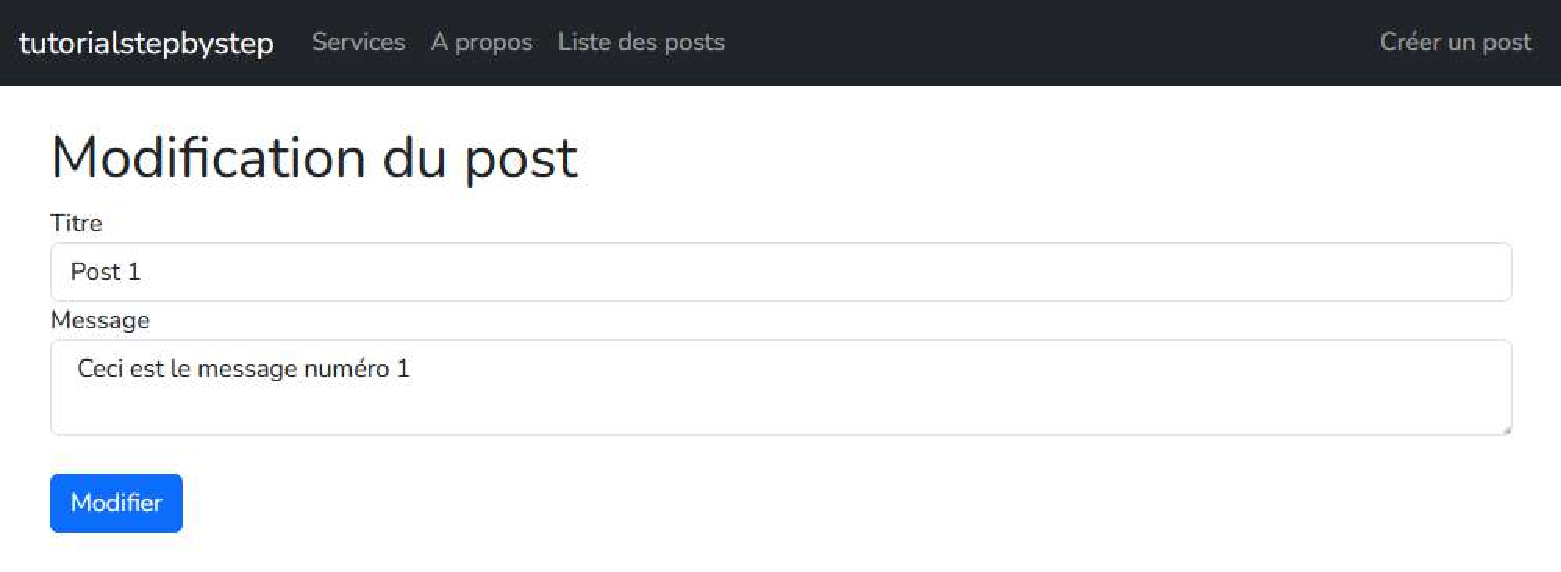
\includegraphics[width=\textwidth]{figures-C1/posts_edit.pdf}}
    \end{subfigure}\hfill
    \begin{subfigure}[c]{0.24\textwidth}
        \caption{\url{http://tutorialstepbystep/posts/1/edit}}
    \end{subfigure}
    \caption{Les quatres pages de gestions des posts.}
\end{figure}

\newpage
